\documentclass[a4paper]{article}

%% Language and font encodings
\usepackage[utf8x]{inputenc}
\usepackage[T1]{fontenc}
\usepackage{polski}

%% Sets page size and margins
\usepackage[a4paper,top=3cm,bottom=2cm,left=3cm,right=3cm,marginparwidth=1.75cm]{geometry}

%% Useful packages
\usepackage{amsmath}
\usepackage{graphicx}
\usepackage[colorinlistoftodos]{todonotes}
\usepackage[colorlinks=true, allcolors=blue]{hyperref}

\title{Dokumentacja końcowa MBI - Analizy populacyjne}
\author{Artur M. Brodzki, Adam Małkowski}

\begin{document}
\maketitle

\section{Wstęp}
W ramach projektu wykonaliśmy aplikację umożliwiającą wykonanie analizy populacyjnej na wczytywanych z wejścia plikach VCF lub GDS. Na wczytywanych danych wykonywana jest analiza PCA, a wyniki prezentowane są w postaci wykresu 2D. Oprócz tego, na danych genetycznych wykonujemy grupowanie metodą hierarchiczną a następnie analizujemy uzyskane wyniki pod kątem zgodności grupowania z deklarowaną grupą etniczną badanych osób. Kod aplikacji jest napisany w języku R, w środowisku R-Studio i wykorzystuje pakiet SNPRelate, umożliwiający łatwe wykonanie analizy populacyjnej na danych genetycznych w formatach VCF oraz GDS. Interfejs aplikacji zrealizowany jest w formie aplikacji webowej, napisanej we frameworku Shiny. 

\section{Funkcjonalność aplikacji}

\begin{figure} \label{fig:empty}
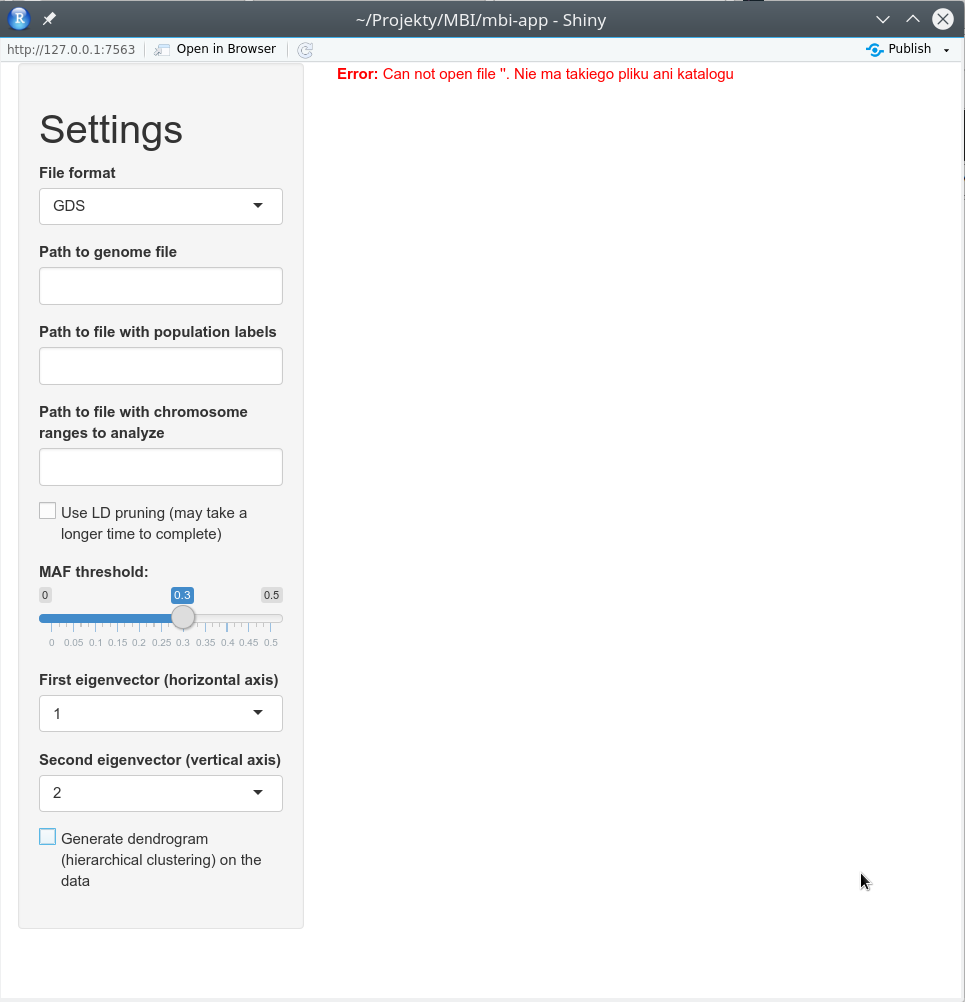
\includegraphics[width=10cm]{empty-files.png}
\centering \caption{Główny interfejs aplikacji bezpośrednio po uruchomieniu.}
\end{figure}

Podstawowy interfejs aplikacji zaprezentowany jest na rys. \ref{fig:empty}. Aplikacja posiada dwa panele: panel lewy odpowiada za ustawienia parametrów, po prawej stronie pojawiają się stosowne wykresy. Możliwe jest dostosowanie następujących ustawień:
\begin{itemize}
\item Format wczytywanych plików: dostępne są formaty VCF oraz GDS. Ze względu na brak jakiejkolwiek kompresji czy choćby optymalizacji sposobu przechowywania danych w plikach VCF, potrafią one osiągać znaczne rozmiary i czasy przetwarzania. Format GDS jest formatem natywnym dla pakietu SNPRelate i zalecana jest praca z plikami w tym właśnie formacie. W przypadku wczytywania pliku VCF, wykonywana jest najpierw konwersja do odpowiadającego mu pliku GDS, co potrafi trwać kilkanaście minut. 
\item Plik z danymi populacyjnymi (populacje referencyjne): W tym pliku powinny być zawarte informacje nt, przynależności badanych osobników do określonych populacji; pliki takie są dostępne do pobrania razem z informacjami o chromosomach w witrynie projektu 1000genomes. 
\end{itemize}
Ustawienie pliku z danymi genetycznymi i referencyjnymi populacjami, pozwala już wygenerować na ich podstawie wykres PCA, widoczny na rys. \ref{fig:pca}. 

\begin{figure}
\centering 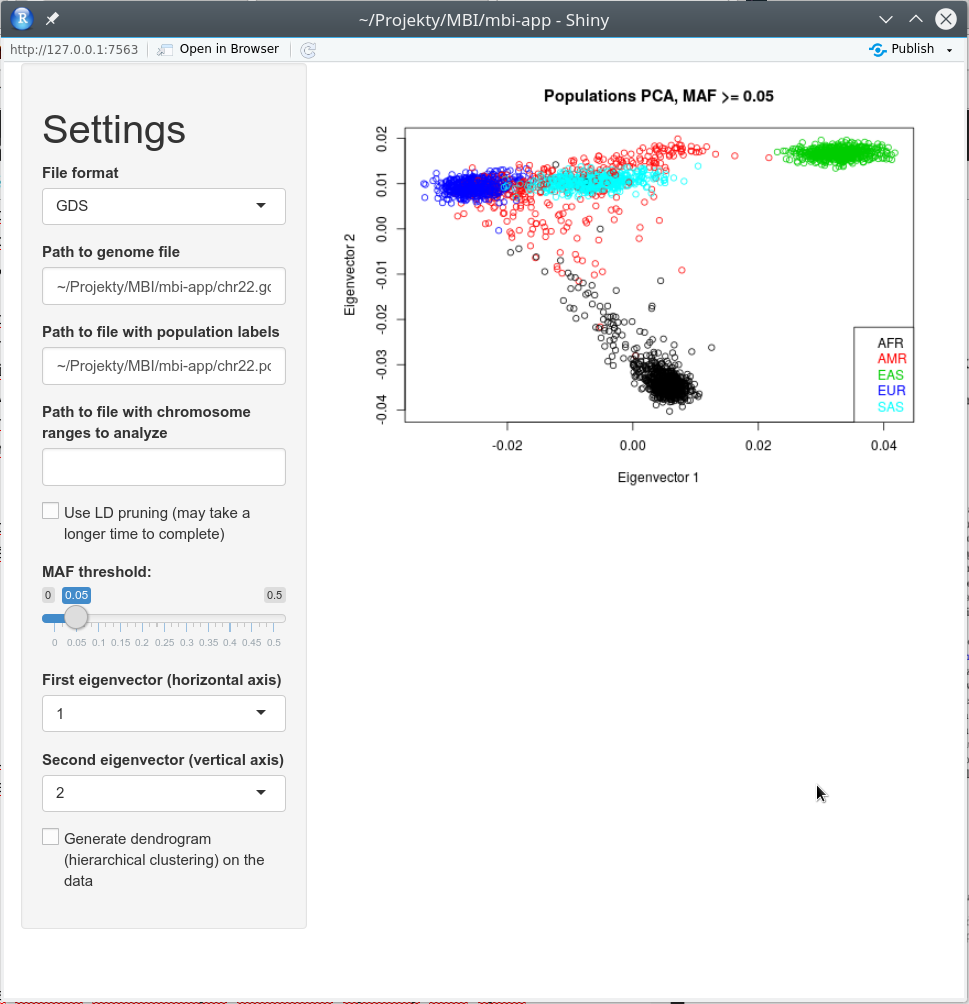
\includegraphics[width=10cm]{example-pca.png}
\caption{Przykładowy wykres PCA.} \label{fig:pca}
\end{figure}

\begin{itemize}
\item Zakres badanych alleli: Parametr opcjonalny. Jeżeli jest ustawiony, wczytywany jest plik TSV zawierający zakres(y) alleli, które będą analizowane. 
\item LD-pruning: czyli przycinanie składowych sprzężonych - włączenie tej opcji wykonuje na danych algorytm LD-pruning, czyli usuwa allele, których występowanie nie jest statystycznie niezależne. Taka operacja może poprawić wyniki działania algorytmu PCA ze względu na eliminację redundantnych korelacji w danych. 
\item Próg MAF (ang. \emph{minimal allel frequency}): zmiana tej wartości pozwala wybrać do analizy jedynie allele o pewnej minimalnej częstotliwości występowania. 
\item Składowe wykresu PCA: analiza PCA generuje zbiór składowych najlepiej wyjaśniających zmienność analizowanych danych. Składowe numerowane są przez $1..n$ w kolejności malejącej: składowa 1 wyjaśnia największy procent zmienności danych, a składowa $n$ najmniejszy. Ponieważ wykres PCA jest dwuwymiarowy, istnieje możlwość wyboru, które składowe PCA są prezentowane na wykresie; domyślnie jest to pierwsza i druga składowa. 
\item Grupowanie hierarchiczne: gdy włączona jest opcja generowania dendrogramu, na danych genetycznych wykonywane jest grupowanie hierarchiczne. Powstałe drzewo obcinane jest do 5 grup (tyle, ile głównych grup etnicznych) a dane prezentowane na wykresie - dendrogramie. Przykładowy dendrogram widoczny jest na rys. \ref{fig:dend}. 
\end{itemize}

\begin{figure}
\centering 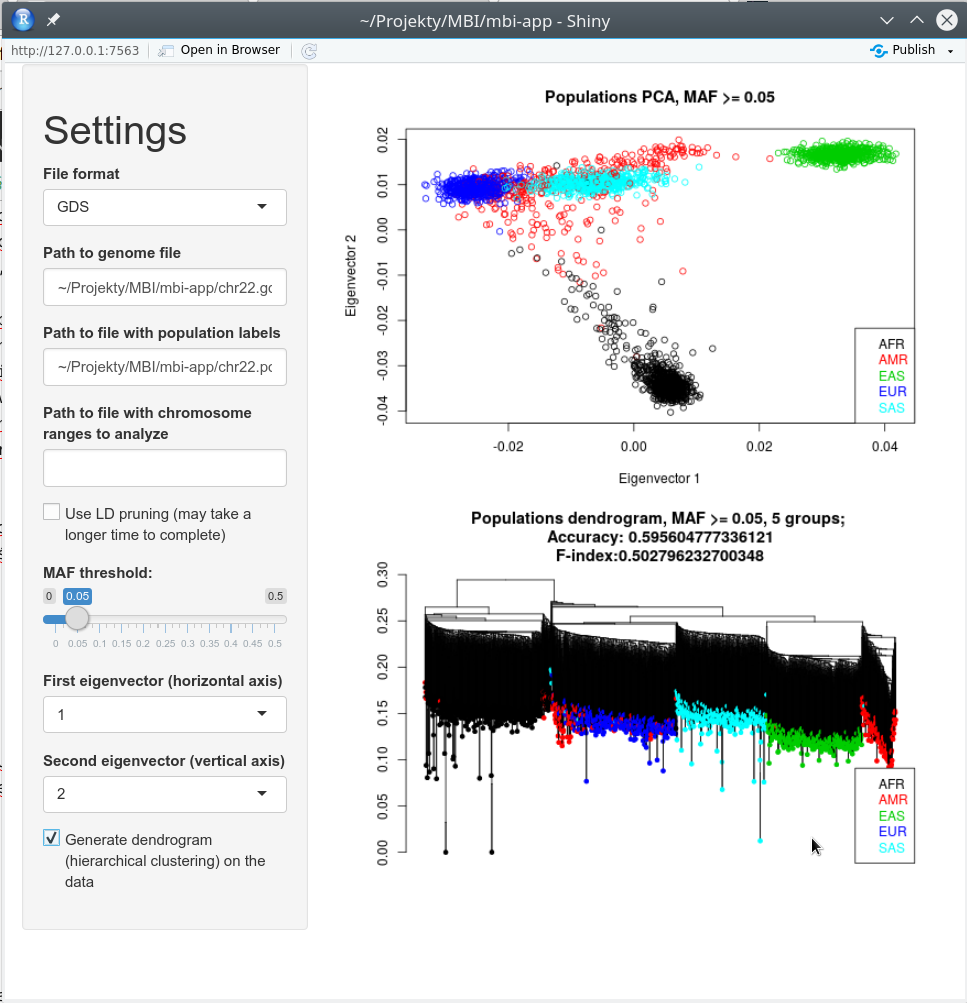
\includegraphics[width=10cm]{example-dend}
\caption{Przykładowy wynik grupowania hierarchicznego, generowany przy włączonej opcji \emph{Generate dendrogram}.} \label{fig:dend}
\end{figure}

\section{Testy}
Przeprowadziliśmy testy działania aplikacji dla różnych wartości parametrów algorytmu PCA oraz sprawdziliśmy jakość uzyskanego grupowania. Jako dane genetyczne służące do testowania aplikacji wykorzystaliśmy dane udostępniane przez projekt 1000genomes na stronie \url{http://www.internationalgenome.org/data}. Wykorzystaliśmy dane fazy 3 projektu, ponieważ zawierają one największą liczbę wariantów SNP - aż 84,4 mln - uzyskanych od 2504 osób. Ponieważ dane genetyczne osiągają znaczne rozmiary (pliki VCF dla całego genomu i 2500 osób mogą sięgać setek GB), nasze analizy ograniczyliśmy do chromosomu 22, który jest najmniejszym chromosomem autosomalnym. Pomimo tego, plik VCF zawierający wszystkie dane dotyczące tego chromosomu zajmuje 10,5GB a jego wstępne przetworzenie zajmuje na komputerze klasy PC kilkanaście minut. 

Dane udostępniane przez projekt 1000genomes dostarczają informacji nt. powiązań alleli z etnicznością badanych osób. Analizowanych jest 5 głównych grup etnicznych:
\begin{itemize}
\item Afrykańska (AFR)
\item Amerykańska (AMR)
\item Bliskowschodnia (EAS)
\item Europejska (EUR)
\item Azja Południowo-Wschodnia (SAS)
\end{itemize}
5 głównych grup etnicznych, odpowiadających z grubsza poszczególnym kontynentom, podzielone jest na 26 mniejszych, regionalnych populacji, jednak w naszym projekcie analizujemy dane jedynie pod kątem głównych grup etnicznych. 

Najważniejsze wnioski z przeprowadzonych testów są następujące:
\begin{enumerate}
\item Parametrem decydującym o uzyskanych wynikach jest próg MAF. Dla małych wartości, niemal wszystkie allele są wykorzystywane w analizie i wyniki są o wiele bardziej dokładne (rys. \ref{fig:ld}). Dla MAF >= 0.45 wykorzystywana liczba alleli jest na tyle mała, że algorytm PCA nie potrafi wyodrębnić na wykresie poszczególnych grup etnicznych (rys. \ref{fig:maf05-ld}). 
\item Analogiczne zjawisko zachodzi dla małej liczby alleli, wynikającej z wybrania wąskiego zakresu analizowanego chromosomu w opcjonalnym pliku TSV. 
\item Algorytm LD-pruningu (rys. \ref{fig:ld}) wpływa na wyniki w mniejszym bądź większym stopniu, zależnie od wartości parametru MAF:
\begin{enumerate}
\item Dla małych wartości MAF, nie zmienia zasadniczo wyniku analizy PCA (rys. \ref{fig:nold} oraz \ref{fig:ld}), za to skraca czas wykonania algorytmu PCA. Jego wpływ na całkowity czas wykonania analizy jest jednak dyskusyjny: o ile czas samej analizy PCA spada dzięki zastosowaniu \emph{LD-pruningu} ok. 10-krotnie, o tyle sam \emph{LD-pruning} zajmuje znaczną ilość czasu, przez co sumaryczny wynik złożoności czasowej jest porównywalny. Być może wyniki byłyby inne dla większych danych wejściowych. 
\item Dla dużych wartości MAF i małych ilości wykorzystywanych w analizie alleli, sytuacj wygląda inaczej. Na częstych allelach uwidacznia się w sposób szczególnie wyraźny cecha algorytmu \emph{LD-pruning} polegająca na usuwaniu redundantnych korelacji. Bez wykorzystania \emph{LD-pruningu}, widoczne są wyraźnie silne, liniowe korelacje pomiędzy allelami (rys. \ref{fig:maf0.5-nold}, które znikają po zastosowaniu \emph{LD-pruningu} (rys. \ref{fig:maf05-ld} a wyniki są bardziej jednorodne. 
\end{enumerate}
\item Pomiary jakości grupowania hierarchicznego okazały się zaskakujące. Do pomiaru jakości grupowania wykorzystaliśmy dwa wskaźniki: skuteczność (ang. \emph{accuracy}) wyrażaną z procentach oraz klasyczny F-indeks. 

W tym wypadku, podobnie jak dla PCA, decydującym parametrem jest MAF; dla jego dużych wartości nie można spodziewać się skutecznego grupowania (rys. \ref{fig:dend-05}): skuteczność wyniosła 56 \%, a F-indeks jesdynie 0.43. Pewnym zaskoczeniem były jednak wyniki grupowania przy wykorzystaniu niemal wszystkich alleli (MAF 0.05). Wyniki tego grupowania prezentuje rys. \ref{fig:dend-005}. 

O ile graficznie wykres wydaje się o wiele bardziej uporządkowany, i można spodziewać się znacznego wzrostu jakości grupowania - to skuteczność wzrasta jedynie do 59\%, a F-indeks do 0.5. Interesująca wydaje się analiza przyczyn takiego stanu rzeczy. Zarówno na wykresach PCA, jak i na dendrogramie \ref{fig:dend-005} widoczna jest znaczna zmienność genetyczna populacji AMR (amerykańskiej). O ile pozostałe grupy etniczne na wykresach PCA tworzą dość zwarte grupy, o tyle grupa amerykańska posiada licznych przedstawicieli o genomie podobnym do europejskiego, azjatyckiego oraz afrykańskiego. Przyczyna tego leży zapewne w historii współczesnej Ameryki:
\begin{enumerate}
\item Jako byłe państwo kolonialne, pierwsi osadnicy w Ameryce byli pochodzenia europejskiego
\item usankcjonowane niewolnictwo oraz handel ludźmi w XIX wieku doprowadziły do sprowadzenia na kontynent amerykański znacznej ilości osób czarnoskórych. Po wprowadzeniu przez prezydenta Lincolna powszechnej abolicji, wielokrotnie dochodzi do zawierania mieszanych małżeństw, co widoczne jest w wykresach PCA w postaci czerwonej "ścieżki" prowadzącej od centrum grupy etnicznej AMR w stronę grupy AFR. 
\item Znaczny poziom życia, zapewniany przez amerykańską gospodarkę, przyciągał do USA wielu imigrantów z kontynentalnych Chin, zwłaszcza na przełomie XIX i XX wieku. Widoczne jest to w niewielkiej odległości obszaru SAS od AMR na wykresach PCA. 
\end{enumerate}
Mieszanie populacji wpływa na mieszanie alleli i z pewnością utrudnia wykonanie klasycznego grupowania zgodnego z deklarowaną przez osoby badane grupą etniczną. 


\end{enumerate}

\begin{figure} 
\centering 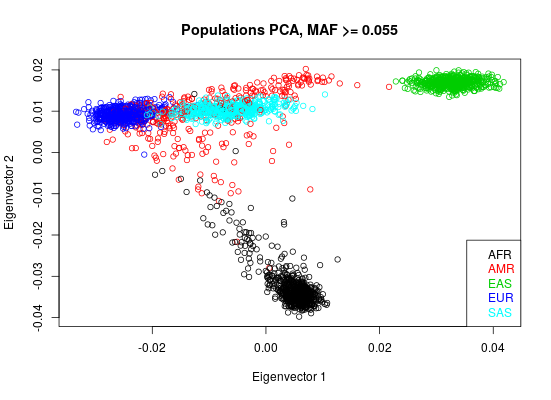
\includegraphics[width=13cm]{pca-nold.png}
\caption{Wykres PCA dla MAF $\geq$ 0.05, bez \emph{LD-pruning}. } \label{fig:nold}
\end{figure}

\begin{figure}
\centering 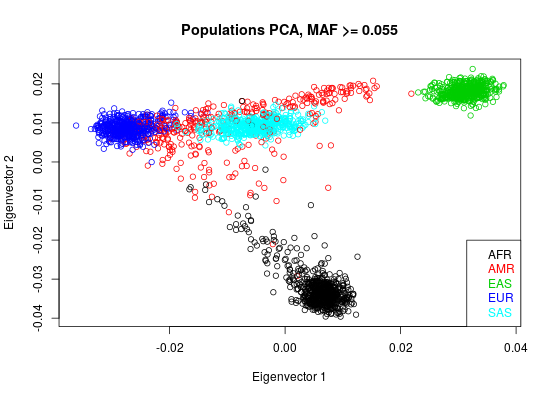
\includegraphics[width=13cm]{pca-ld.png}
\caption{Wykres PCA dla MAF $\geq$ 0.05, po wykonaniu algorytmu \emph{LD-pruning}. } \label{fig:ld}
\end{figure}

\begin{figure} 
\centering 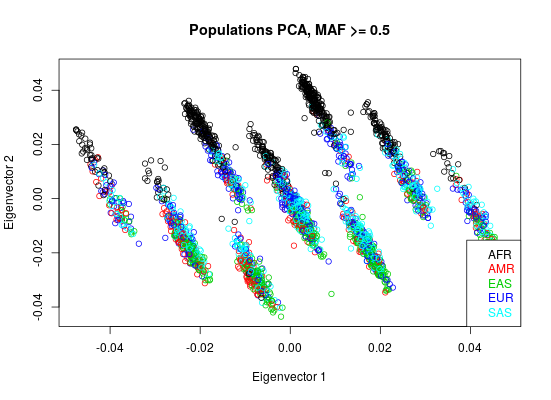
\includegraphics[width=13cm]{pca-maf-0_5-nold.png}
\caption{Wykres PCA dla MAF $\geq$ 0.5, bez \emph{LD-pruning}. } \label{fig:maf0.5-nold}
\end{figure}

\begin{figure}
\centering 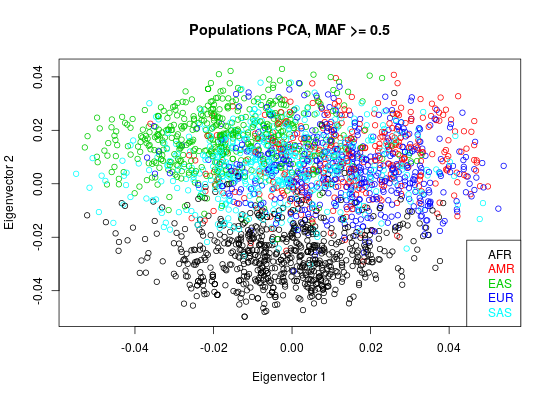
\includegraphics[width=13cm]{pca-maf-0_5.png}
\caption{Wykres PCA dla MAF $\geq$ 0.5, po wykonaniu algorytmu \emph{LD-pruningu}. } \label{fig:maf05-ld}
\end{figure}

\begin{figure} 
\centering 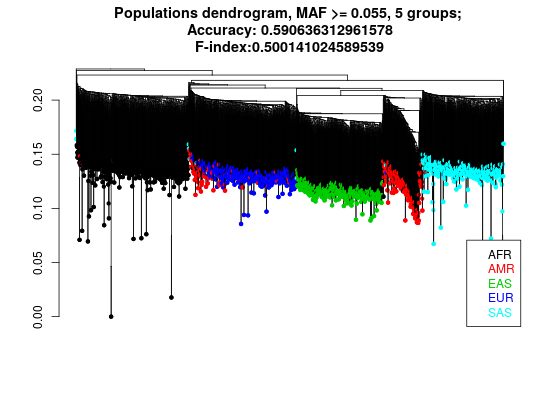
\includegraphics[width=13cm]{dend-maf-0_05-ld.png}
\caption{Dendrogram dla MAF $\geq$ 0.05, z użyciem \emph{LD-pruning}. } \label{fig:dend-005}
\end{figure}

\begin{figure}
\centering 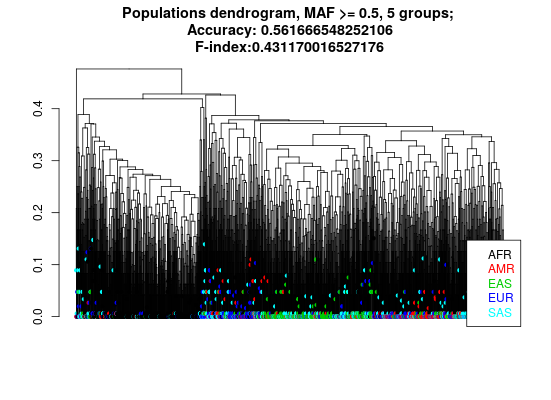
\includegraphics[width=13cm]{dend-maf-0_5-ld.png}
\caption{Wykres PCA dla MAF $\geq$ 0.5, z użyciem \emph{LD-pruningu}. } \label{fig:dend-05}
\end{figure}





\end{document}